
\item \points{25} {\bf Reinforcement Learning: The inverted pendulum}

In this problem, you will apply reinforcement learning to automatically
design a policy for a difficult control task, without ever using any 
explicit knowledge of the dynamics of the underlying system.

The problem we will consider is the inverted pendulum or the pole-balancing 
problem.\footnote{The dynamics are adapted from {\tt
    http://www-anw.cs.umass.edu/rlr/domains.html}}

Consider the figure shown. A thin pole is connected via a free hinge to a cart, 
which can move laterally on a smooth table surface. The controller is said to 
have failed if either the angle of the pole deviates by more than a certain
amount from the vertical position (i.e., if the pole falls over), or if the
cart's position goes out of bounds (i.e., if it falls off the end of the table).
Our objective is to develop a controller to balance the pole with these 
constraints, by appropriately having the cart accelerate left and right.


\begin{center}
  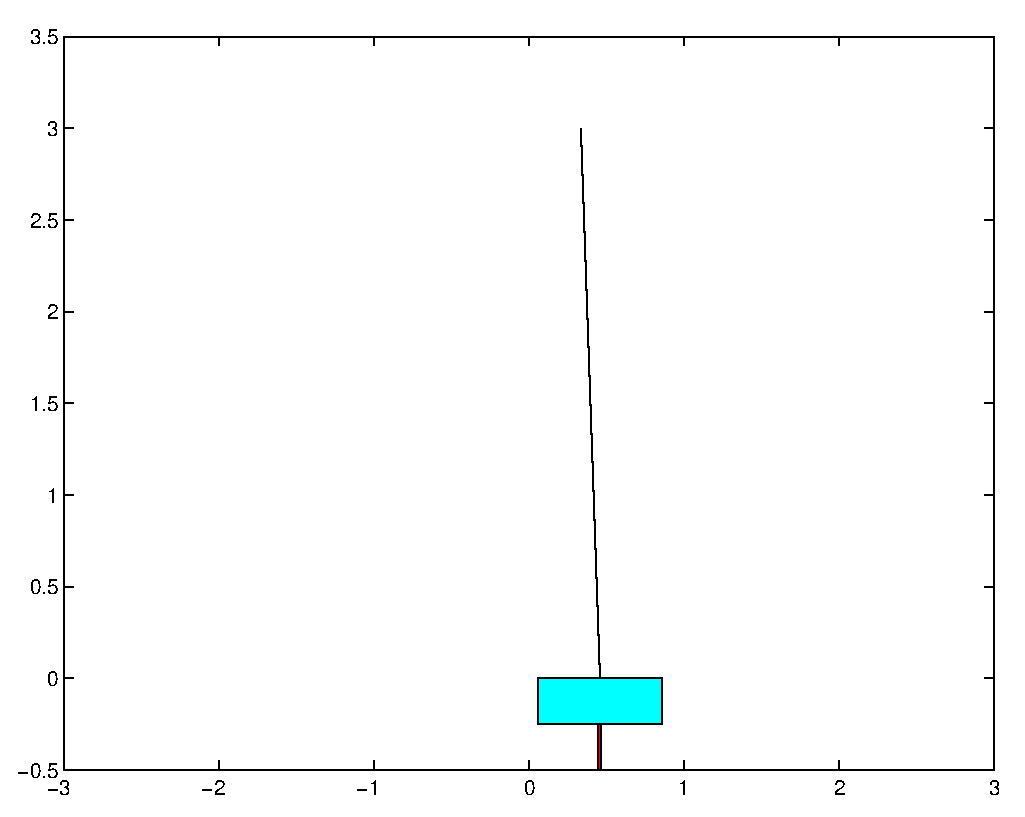
\includegraphics[width=6cm]{cartpole/cart_pole.eps}
\end{center}

We have written a simple simulator for this problem. The simulation 
proceeds in discrete time cycles (steps). The state of the cart and pole at any time 
is completely characterized by 4 parameters: the cart position $x$, the 
cart velocity $\dot{x}$, the angle of the pole $\theta$ measured as its deviation 
from the vertical position, and the angular velocity of the pole $\dot{\theta}$.  
Since it would be simpler to
consider reinforcement learning in a discrete state space,
we have approximated the state space by a discretization that maps 
a state vector $(x,\dot{x}, \theta, \dot{\theta})$ into a number
from 0 to {\tt NUM\_STATES-1}. Your learning algorithm will need to 
deal only with this discretized representation of the states.

At every time step, the controller must choose one of two actions -
push (accelerate) the cart right, or push the cart left.
(To keep the problem simple, there is no {\it do-nothing} action.)
These are represented as actions $0$ and $1$ respectively in the code.  
When the action choice is made, the simulator updates the state parameters 
according to the underlying dynamics, and provides a new discretized state.

We will assume that the reward $R(s)$ is a function of the current state only.
When the pole angle goes beyond a certain limit or when the cart goes
too far out, a negative reward is given, and the system is reinitialized 
randomly. At all other times, the reward is zero.  Your program must learn 
to balance the pole using only the state transitions and rewards observed.

The files for this problem are in {\tt src/cartpole/} directory.
Most of the the code has already been written for you, and you need 
to make changes only to {\tt cartpole.py} in the places specified. This 
file can be run to show a display and to plot a learning curve 
at the end.  Read the comments at the top of the file for more details
on the working of the simulation.

 To solve the inverted pendulum problem, you will estimate a 
  model (i.e., transition probabilities and rewards) for the underlying 
  MDP, solve Bellman's equations for this estimated MDP to obtain
  a value function, and act greedily with respect to this value function.  

  Briefly, you will maintain a current model of the MDP and a current
  estimate of the value function. Initially, each state has estimated reward zero,
  and the estimated transition probabilities are uniform (equally likely 
  to end up in any other state).

  During the simulation, you must choose actions at each time step 
  according to some current policy.  As the program goes along taking 
  actions, it will gather observations on transitions and rewards,
  which it can use to get a better estimate of the MDP model.
  Since it is inefficient to update the whole estimated MDP after every 
  observation, we will store the state transitions and reward observations 
  each time, and update the model and value function/policy only periodically. 
  Thus, you must maintain counts of the total number of times the 
  transition from state $s_i$ to state $s_j$ using action $a$ has been 
  observed (similarly for the rewards).  Note that the rewards at 
  any state are deterministic, but the state transitions are not because 
  of the discretization of the state space (several different but close
  configurations may map onto the same discretized state).

  Each time a failure occurs (such as if the pole falls over), you should 
  re-estimate the transition probabilities and rewards as the average of 
  the observed values (if any).  Your program must then use value iteration 
  to solve Bellman's equations on the estimated MDP, to get the value function 
  and new optimal policy for the new model.  For value iteration, use a 
  convergence criterion that checks if the maximum absolute change in the 
  value function on an iteration exceeds some specified tolerance. 

  Finally, assume that the whole learning procedure has converged 
  once several consecutive attempts (defined by the parameter 
  {\tt NO\_LEARNING\_THRESHOLD}) to solve Bellman's
  equation all converge in the first iteration. Intuitively, this
  indicates that the estimated model has stopped changing significantly.

  The code outline for this problem is already in 
  {\tt cartpole.py}, and you need to write code fragments only at the
  places specified in the file. There are several details (convergence criteria
  etc.) that are also explained inside the code. Use a discount factor
  of $\gamma = 0.995$.  

  Implement the reinforcement learning algorithm as specified, and run it.

\begin{itemize}
\item  How many trials (how many times did the pole fall over or the cart fall off) 
  did it take before the algorithm converged? 
  Hint: if your solution is correct, on the plot the red line indicating smoothed log num 
  steps to failure should start to flatten out at about 60 iterations.

\item  Plot a learning curve showing the number of time-steps for which the
  pole was balanced on each trial. Python starter code already includes the code to plot.
  Include it in your submission.
  
\item  Find the line of code that says np.random.seed, and rerun the code with the seed set to 1, 2, and 3.
       What do you observe? What does this imply about the algorithm?

\end{itemize}

\ifnum\solutions=1 {
  \begin{answer}
\end{answer}

} \fi
